\documentclass{article}
\usepackage[utf8]{inputenc}
\usepackage[hidelinks]{hyperref}
\usepackage{color}
\usepackage{graphics}
\usepackage{graphicx}
\usepackage{amsfonts}
\usepackage{fancybox}
\usepackage[spanish,es-tabla]{babel}

\usepackage[spanish]{babel}

\title{Matemáticas Computacionales \\ Practica 2: Estudio de una Base de Datos}
\author{1860560 Rangel Delgado Jesus Angel}
\date{07 de Marzo del 2021}

\begin{document}

\maketitle

\section{Introducción}
En esta practica estudiaremos una base de datos con estadística descriptiva en R, analizaremos todos los datos que nos proporciona la base de datos como atributos, tipos de dato, etc.
Se detalla todo el procedimiento realizado para la vista de tablas, gráficas, etc.

\section{Base de Datos ChickWeight}
La base de datos que seleccione consiste en el estudio de los pesos corporales de pollitos, partiendo del día 0 y cada dos días, hasta el día 20 ademas también se tomo el peso del día 21
\textbf{Observación:} Los pollitos estaban separados en 4 grupos diferentes y cada grupo estaba sometido a una dieta diferente

\subsection{Observaciones de la base de datos}
En primer lugar observemos en la siguiente la tabla que representa la cantidad de cada grupo de pollitos en base a su dieta
\newpage
\begin{table}[h]
\begin{center}
\begin{tabular}{| r  | c |}
Grupo & Cantidad  \\ \hline
1 & 20  \\
2 & 10 \\
3 & 10 \\
4 & 10 \\ \hline
\end{tabular}
\caption{Cantidad de pollitos por grupo}
\label{tab:pollito}
\end{center}
\end{table}

Entonces observe que de la tabla \ref{tab:pollito} tenemos que en total se trabajaron con 50 pollitos

Ahora el código en r nos genera una tabla con estadística mayormente acertada en los primeros datos de las tablas generadas por la base de datos en R (Los pesos de los pollos)

\begin{figure}[h]
    \centering
    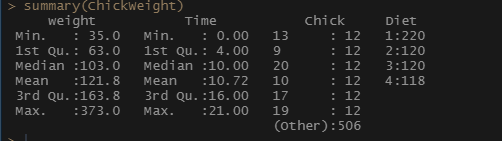
\includegraphics[width=10cm, height=4cm]{P2MC.PNG}
    \caption{Tablas generadas al ejecutar la instrucción summary}
    \label{fig:mesh1}
\end{figure}

Observe que en el primer apartado que corresponde a la tabla de pesos el menor peso registrado es de 35, que al buscarlo en la base de datos propuesta corresponde al pollo numero 18 correspondiente al grupo 1 quien para el día 2 que se hizo la prueba perdió peso
En la siguiente ilustración se muestra lo ya explicado en el párrafo anterior
\newpage

\begin{figure}[h]
    \centering
    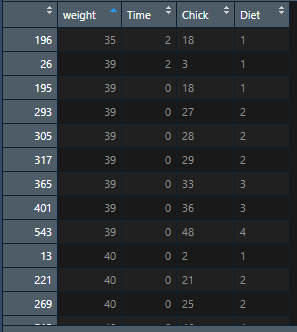
\includegraphics{P2MC2.PNG}
    \caption{Base de Datos ChickWeight en R }
    \label{fig:mesh2}
\end{figure}

Así como el ejemplo anterior, se pueden realizar mas comparativas con los diferentes datos.
\newline
Ahora observamos que la tabla generada con la función \textbf{summary} también nos proporciona otros datos como la Mediana de los datos capturados para los pesos la cual es: \textbf{103}
\newline
\newline
\shadowbox{Observación}
\textbf{¿Que es la mediana?}
\newline
La mediana : es el valor "más céntrico", una vez que los datos se ordenan según su tamaño. Si el número de observaciones es impar, la mediana es el valor de la observación en la posición 
\begin{equation}
    \frac{n+1}{2}
\end{equation}
 y si el número de observaciones es par, la mediana se define como la media (el promedio) de las observaciones en las
posiciones
\begin{equation}
    \frac{n}{2} \hspace{1cm}  y  \hspace{1cm} \frac{n+2}{2}
\end{equation}

Otro dato que también podemos recabar de la tabla ya mostrada anteriormente es la media la cual es igual a \textbf{121.8}

\newpage
\shadowbox{Observación}
\textbf{¿Que es la media?}
\newline
La media : es la suma de las observaciones dividida
entre el tamaño de la muestra o de la población.
\newline
\newline
Otro dato que también nos ofrece la tabla son los cuartiles en su primer y tercer cuartil esto es igual a \textbf{63.0} para el primer cuartil y para el tercero este es igual a \textbf{163.8}

\shadowbox{Observación}
\textbf{¿Que es el cuartil?}
\newline
Los cuartiles: son valores que dividen una muestra de datos en cuatro partes iguales. Utilizando cuartiles puede evaluar rápidamente la dispersión y la tendencia central de un conjunto de datos, que son los pasos iniciales importantes para comprender sus datos.

\begin{itemize}
    \item Primer cuartil: 25\% de los datos es menor que o igual a este valor
    \item Tercer cuartil: 75\% de los datos es menor que o igual a ese valor
\end{itemize} 

Por ultimo la tabla del inicio nos genera el valor máximo de los pesos obtenidos por los pollitos el cual es: \textbf{373} el cual se enuentra ubicado con el pollito numero 35 que esta en el grupo de la dieta 3 y este peso lo presento en el ultimo dia de la prueba

\begin{figure}[h]
    \centering
    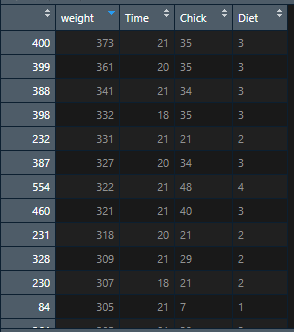
\includegraphics{P2MC3.PNG}
    \caption{Base de Datos ChickWeight en R }
    \label{fig:mesh3}
\end{figure}


\newpage
\subsection{Tablas de Frecuencia}
Antes de comenzar con las gráficas observe que el programa de R también ofrece mas funciones para estadística como la tabla de frecuencias
\newline
Para ejemplificar este apartado decidí obtener la tabla de frecuencias para ver cuanto es el por ciento de pollitos en cada grupo con su dieta.
\begin{table}[h]
\begin{center}
\begin{tabular}{| r  | c |}
Grupo & Porcentaje  \\ \hline
1 & 38.06\%  \\
2 & 20.76\%  \\
3 & 20.76\%  \\
4 & 20.41\%  \\ \hline
\end{tabular}
\caption{Cantidad de pollitos por grupo en porcentaje}
\label{tab:cantidad}
\end{center}
\end{table}

\begin{figure}[h]
    \centering
    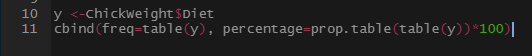
\includegraphics[width=12cm, height=2cm]{P2MC4.PNG}
    \caption{Código en R para generar la tabla de frecuencias }
    \label{fig:mesh4}
\end{figure}

\subsection{Calculo de Correlaciones}
Otra de las funciones que nos ofrece el programa R es poder realizar el calculo de correlaciones
Para ejemplificar este punto realizare la correlación entre el peso de los pollitos y los días que duro el experimento

\begin{table}[h]
\begin{center}
\begin{tabular}{| r  | c |}
Peso & Tiempo  \\ \hline
1.0000000 & 0.8371017 \\
0.8371017 & 1.0000000 \\ \hline
\end{tabular}
\caption{Correlación entre el peso y tiempo}
\label{tab:correlacion}
\end{center}
\end{table}

\newpage
\begin{figure}[h]
    \centering
    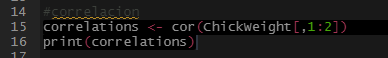
\includegraphics{P2MC5.PNG}
    \caption{Código en R para generar la Correlación }
    \label{fig:mesh5}
\end{figure}

\shadowbox{Observación}
\textbf{¿Que es la correlación?}
\newline
La Correlación: indica la fuerza y la dirección de una relación lineal y proporcionalidad entre dos variables estadísticas. Se considera que dos variables cuantitativas están correlacionadas cuando los valores de una de ellas varían sistemáticamente con respecto a los valores homónimos de la otra: si tenemos dos variables (A y B) existe correlación entre ellas si al disminuir los valores de A lo hacen también los de B y viceversa. La correlación entre dos variables no implica, por sí misma, ninguna relación de causalidad 

\section{Gráficas de la base de datos}
Otra de las ventajas de trabajar bases de datos en R es que podemos realizar graficas con todos los datos que estemos trabajando, a continuación unos ejemplos:
\subsection{Histogramas}
\shadowbox{Observación}
\textbf{¿Qué es un histograma?}
\newline
El histograma: es un gráfico de rectángulos que tiene su base en el eje x, de igual ancho cuando representa el comportamiento de una variable discreta, o de anchura proporcional a la longitud del intervalo cuando se desea representar una variable continua. En
este último caso el punto central de la base de los rectángulos equivale al punto medio de cada clase
\newline
Ejemplo de un Histograma:
\begin{figure}[h]
    \centering
    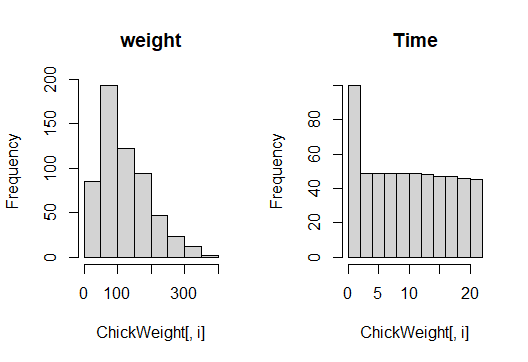
\includegraphics[width=10cm, height=4cm]{Histograma.png}
    \caption{Histograma en base a los pesos y el tiempo }
    \label{fig:mesh6}
\end{figure}

\newpage
\begin{figure}[h]
    \centering
    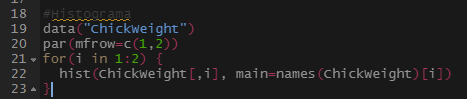
\includegraphics[width=12cm, height=4cm]{P2MC6.PNG}
    \caption{Código para generar el histograma }
    \label{fig:mesh7}
\end{figure}

\subsection{Gráfica de correlaciones}
Ejemplo de una Gráfica de Correlación:
\begin{figure}[h]
    \centering   
    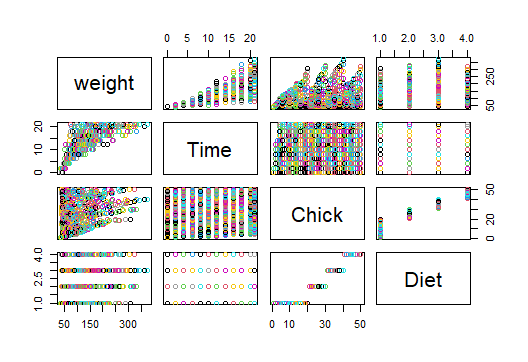
\includegraphics[width=10cm, height=4cm]{Grafica de Correlaciones.png}
    \caption{Gráfica de Correlación en base a los pesos y el tiempo }
    \label{fig:mesh8}
\end{figure}
\begin{figure}[h]
    \centering
    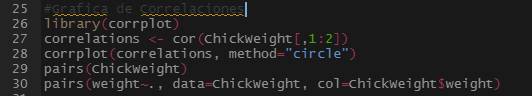
\includegraphics[width=10cm, height=2cm]{P2MC7.PNG}
    \caption{Código para generar las gráficas de correlaciones  } 
    \label{fig:mesh9}
\end{figure}

\subsection{Gráficos de densidad por clase}
Otro de los gráficos que nos proporciona el programa de R es el de crear gráficos de densidad por clase para ejemplificar esto decidí hacer un gráfico del tiempo y peso con respecto a la dieta
\newpage
\shadowbox{Observación}
\textbf{¿Qué es un Gráfico de densidad?}
\newline
El gráfico de densidad: visualiza la distribución de datos en un intervalo o período de tiempo continuo. Este gráfico es una variación de un Histograma que usa el suavizado de cerner para trazar valores, permitiendo distribuciones más suaves al suavizar el ruido. Los picos de un gráfico de densidad ayudan a mostrar dónde los valores se concentran en el intervalo.

\begin{figure}[h]
    \centering
    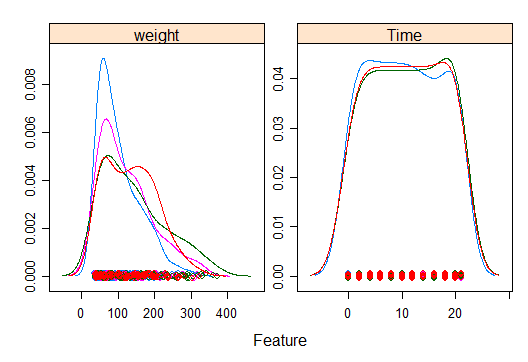
\includegraphics[width=10cm, height=4cm]{Graficos de densidad por clase.png}
    \caption{Gráfica de densidad por clase }
    \label{fig:mesh10}
\end{figure}

\begin{figure}[h]
    \centering
    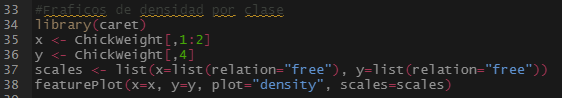
\includegraphics[width=10cm, height=2cm]{P2MC8.PNG}
    \caption{Código para generarlas gráficas de densidad por clase  }
    \label{fig:mesh11}
\end{figure}

\subsection{Diagramas de caja}
Por ultimo veremos un ejemplo del diagrama de caja otro gráfico que nos facilita el estudio de la base de datos
\newline
\shadowbox{Observación}
\textbf{¿Qué es un diagrama de caja?}
\newline
El diagrama de caja: es un gráfico utilizado para representar una variable cuantitativa (variable numérica). El gráfico es una herramienta que permite visualizar, a través de los cuartiles, cómo es la distribución, su grado de asimetría, los valores extremos, la posición de la mediana, etc.
\newline
\newline
Para esté apartado realice dos ejemplos donde observamos el diagrama de caja en base al peso y la dieta asignada y en el segundo caso observemos que el gráfico esta diseñado con respecto al peso y el pollo.


\newpage
\begin{figure}[h]
    \centering
    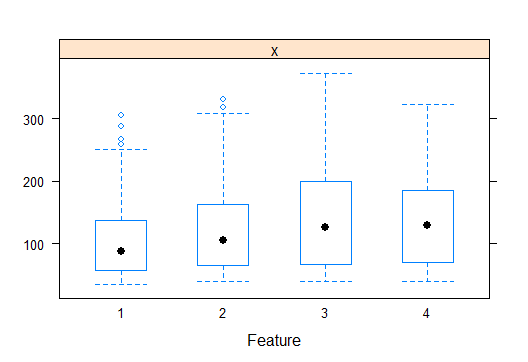
\includegraphics[width=10cm, height=6cm]{Diagramas de caja.png}
    \caption{Diagrama de caja 1}
    \label{fig:mesh12}
\end{figure}

\begin{figure}[h]
    \centering
    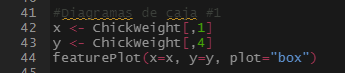
\includegraphics[width=10cm, height=2cm]{P2MC9.PNG}
    \caption{Código para el diagrama de caja 1  }
    \label{fig:mesh13}
\end{figure}

\begin{figure}[h]
    \centering
    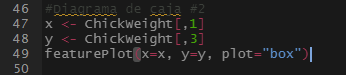
\includegraphics[width=10cm, height=2cm]{P2MC10.PNG}
    \caption{Código para el diagrama de caja 2  }
    \label{fig:mesh14}
\end{figure}

\newpage
\begin{figure}[h]
    \centering
    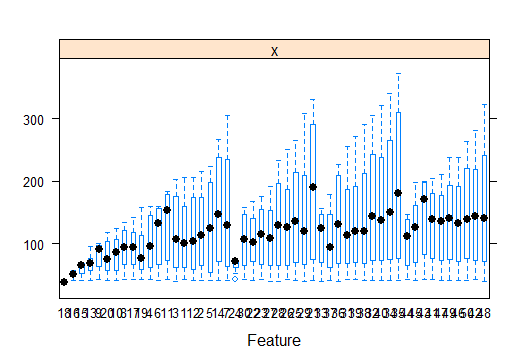
\includegraphics[width=12cm, height=6cm]{Diagrama de caja2.png}
    \caption{Diagrama de cajas 2 }
    \label{fig:mesh15}
\end{figure}

\section{Conclusión}
Como conclusiones de la base de datos observe que los pollitos que  que registraron el mayor peso se encuentran en el grupo que consumió la dieta 3 y los pollitos con el menor peso la mayoría pertenecen a los que consumieron la dieta 1, además también podemos observar como algunos pollitos desde el inicio del consumo de la dieta 1 perdieron peso, lo cual se ejemplifico anteriormente en el documento
Otra cosa que también podemos concluir es que el pollo con el mayor peso es el registrado con el número 35 (pertenece a la dieta 3) y el de menor peso al finalizar el experimento es el registrado con el número 24 (pertenece a la dieta 2).
Otra cosa que también puede ser notoria es que un pollito del grupo de la dieta 4 no logro terminar el experimento ya que después del día 18 no se toma registro alguno de esto este pollito estaba nombrado como 44. Esto es notorio en base la cantidad de datos al finalizar la prueba.
Como conclusión de la practica fue muy interesante observar las ventajas que te ofrece el programa de R para trabajar la estadística, es una muy buena base, para trabajar numerosas cantidades de datos ya que existen muchas funciones que te ayudan a resumir datos que trabajando a mano seria una tarea muy tediosa.

\newpage
\begin{thebibliography}{0}
  \bibitem{Estadisitca matematica con aplicaciones, 2000} Jhon E. Freund, Estadística matemática con aplicaciones, 2000
  \bibitem{R-core R-core@R-project.org, Datasets} Datasets \textcolor{blue}{\url{https://www.rdocumentation.org/packages/datasets/versions/3.6.2}}\href{https://www.rdocumentation.org/packages/datasets/versions/3.6.2}{\textcolor{blue}{Datasets}}
  \bibitem{Jesus Rangel, Repositorio de GitHub}Jesus Rangel, repositorio de GitHub\textcolor{blue}{\url{https://github.com/JesusRangel07/MatematicasComputacionales}}\href{https://github.com/JesusRangel07/MatematicasComputacionales}{\textcolor{blue}{Repositorio de Github}}
\end{thebibliography}



\end{document}
